\begin{problem}{산림의 수호자}{standard input}{standard output}{1 second}{1000 megabytes}

  \it{근성은 나무에 관심이 많다.}


드루이드 근성은 \bf{트리}를 관리하는 '산림의 수호자'이다. 근성이 관리하는 \bf{트리}는 사이클이 없는 단순 연결 그래프 형태로 이루어져 있고, 얼마나 관리가 잘 됐는지 무려 $N$개나 되는 정점을 가지고 있다. 근성은 모든 정점을 소중하게 여겨서 $N$개의 정점들에 각각 $1$에서부터 $N$까지의 고유한 정점 번호를 일일히 매겨놓았다.


어느 날, 근성의 멋진 \bf{트리}를 항상 시기해 오던 사악한 악당 영도가 근성의 \bf{트리}에 불을 지르고 말았다! 근성이 \bf{트리}를 최대한 온전히 보존하기 위해선, \bf{트리}가 완전히 타서 없어지기 전에 \bf{트리}의 각 정점에 저장된 데이터들을 최대한 많이 복제해야 한다.


\begin{itemize}
  \item 초기에 영도는 $a$번 정점을 불태웠고, 근성은 $b$번 정점 위에 서 있다. $(a \neq b)$
\end{itemize}


근성은 불에 타지 않은 정점 위에서 다음 행동 중 하나를 선택하여 수행할 수 있다.


\begin{itemize}
  \item \bf{복제하기}: 근성이 현재 정점에서 데이터를 복제한다. 이 행동은 시간을 소모하지 않는다. 단, 데이터를 이미 복제한 정점에서는 다시 데이터를 복제할 수 없다.
  \item \bf{이동하기}: 근성이 현재 정점에서 간선을 따라 이웃한 불에 타지 않은 정점 중 한 곳으로 이동한다.
  \item \bf{기다리기}: 근성이 현재 정점에서 이동하지 않고 대기한다.


만약 근성이 \bf{이동하기} 또는 \bf{기다리기}를 선택했다면, 수행하는 시간 동안 간선을 따라 이웃한 정점들에 불이 옮겨붙는다. 다시 말해, 불에 타지 않은 정점 중 불타는 정점과 간선을 따라 이웃한 모든 정점에 불이 옮겨붙는다.


만약 근성이가 다음 행동으로 불타는 정점 위에 있게 된다면, 그 즉시 근성은 더 이상의 \bf{트리} 보존 작업을 포기하고 \bf{트리}에서 탈출할 것이다. 근성이가 정점에 도착함과 동시에 해당 정점으로 불이 옮겨붙는다면, 근성은 해당 정점에서 데이터를 복제할 수 없다.


당신이 해야 할 일은 근성이 탈출하기 전까지 데이터를 복제할 수 있는 bf{트리}의 정점 개수의 최댓값을 구하여 근성이에게 알려주는 것이다. 산림의 수호자 근성을 도와 사악한 악당 영도의 계획을 저지해 보자!

\InputFile
첫째 줄에 \bf{트리}의 정점의 개수 $N$$(2 ≤ N ≤ 100000)$이 주어진다.


다음 $N-1$개의 줄에 \bf{트리}의 간선 정보가 각 줄마다 두 정점의 번호 $u$, $v$로 공백으로 구분되어 주어지는데, 정점 $u$와 $v$ 사이에 간선이 존재함을 나타낸다.


그다음 줄에는 최초로 불타는 정점 $a$와 근성이 위치한 정점 $b$의 번호가 한 줄에 각각 공백으로 구분되어 주어진다.

\OutputFile
가능한 모든 경우들 중 근성이 탈출하기 전까지 \bf{트리}에서 데이터를 복제할 수 있는 최대 정점 개수를 출력한다.

\Examples

\begin{example}
\exmpfile{example.01}{example.01.a}%
\exmpfile{example.02}{example.02.a}%
\exmpfile{example.03}{example.03.a}%
\end{example}

\Note
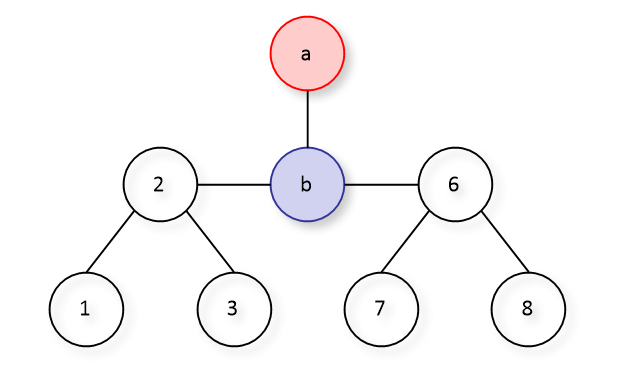
\includegraphics{sot-ex1pic.png}


다음 그림은 \bf{예제 입력 1}에서 주어진 \bf{트리}의 모습이다. 이 문제에서 '\bf{트리}'란 사이클이 없는 단순 연결 그래프를 의미하며, 여기서 '사이클'이란 어느 한 정점에서 출발해 같은 정점을 두 번 이상 방문하지 않고 시작점으로 돌아올 수 있는 경로를 말한다. 주어진 예제 그림은 '사이클이 없는 단순 연결 그래프'의 모습을 만족하고 있다.


이 예제의 경우 근성이 복제할 수 있는 정점 데이터의 최대 개수는 3개이다. 근성이 가능한 최적의 행동 중 하나는, \bf{기다리기}를 사용하지 않고 4(b)-2-1로 이동하며 매 정점마다 \bf{복제하기}를 사용하는 것이다.

\end{problem}

